\section{Notation und Begrifflichkeiten}
In diesem Kapitel werden Notationen bezüglich Teilfolgen, Gewichtung und Sequenzierungen eingeführt. Im zweiten Teil wird dann auf Begriffe aus der Programmierung und Theoretischen Informatik eingegangen.

\subsection{Notation}
\subsubsection{(Teil-)Folgen}
Sei $(a_n)_{n\in\mathbb{N}}$ eine Folge an Buchstaben $a$ über einem Alphabet $\Sigma$ (im weiteren betrachten wir nur die natürlichen Zahlen $\mathbb{N}$ oder andere geordnete Mengen). Wir nennen $(a_n)$ endlich, falls es ein $n\in\mathbb{N}$ gibt, so dass für alle $k\leq n$ $a_k$ definiert ist, und sonst nicht. Im Folgenden werden wir endliche Folgen mit $a_1a_2a_3$\dots$a_n$ notieren. Man nennt eine Folge streng monoton steigend, wenn $a_i < a_{i+1}$ für alle $1\leq i < n$ gilt.\\
Eine Teilfolge von $(a_n)$ ist eine Folge $(b_k)$ für die es $i_1<i_2<$\dots$<i_k$ gibt, s.d.$a_{i_1}a_{i_2}a_{i_3}$\dots$a_{i_k}$ gleich $(b_k)$ entspricht. Betrachtet man $4,3,6,8,1,5$, so wäre $4,6,8$ mit $i_1=1,i_2=3,i_3=4$ eine streng monoton steigende Teilfolge.

\subsubsection{Gewichtungen}
Eine Gewichtungs-Funktion ist eine Zuordnungsfunktion $\Omega:\Sigma\rightarrow\mathbb{N}$ eines Alphabets $\Sigma$ auf die natürlichen Zahlen. Im Allgemeinen werden wir iuns n dieser Arbeit auf den Wert der Zahlen als Gewicht beziehen, die Gewichtsfunktion wäre damit die Identität $Id_\mathbb{N}:x \mapsto x$. Jedoch können auch andere Funktionen für das Gewicht hergenommen werden für die Algorithmen. Diese Gewichtung dient auch als Erweiterung für die Monotonie, statt $a_i<a_{i+1s}$, kann man auch $\Omega (a_i) < \Omega (a_{i+1})$ schreiben. 

\subsubsection{'Rechteck'}
Gegeben seien zwei Paare $s:=(a,b)$ und $t:=(x,y)$ aus $\mathbb{N}^2$ mit $a<x,b<y$. Das Rechteck $(s,t)$ bestehend aus den vier Punkten $(a,b),(a,y),(x,b),(x,y)$ werden wir anhand des kartesischen Produktes $[a,b]\times [x,y] \subset \mathbb{N}^2$ bezeichnen.\\
Wir nennen zwei Rechtecke $o:=(s,t)$ und $p:=(u,v)$ nicht überlappend \\($o\ll p$), g.d.w. $t.x_1<u.x_1$ und $t.x_2 < u.x_2$ gilt, das heißt, das Rechteck $u$ ist $"$oben rechts$"$ von $t$ aus liegend. Eine Kette (Chain) solcher Rechtecke $o_1,\dots ,o_n$ ist ebenso nicht überlappend, falls $o_i \ll o_{i+1} ~ \forall 1\leq i< n$ gilt. Es handelt sich hierbei nicht um eine Ordnung im eigentlichen Sinne, denn für die zwei Rechtecke $s=((1,1),(2,2))$ und $t=((2,1),(3,3))$ gilt nicht $s\ll t$, da $(2,2) < (2,1)$ nicht gilt, $t\ll s$ aber auch nicht, da $(3,3) < (1,1)$ nicht gilt. Bei einer Kette an solchen Rechtecken ist also eine Richtung nach $"$oben rechts$"$ gegeben.

\subsection{Begriffe und Datenstrukturen}
In dieser Arbeit wird immer wieder auf verschiedene Datenstrukturen verwiesen, die hier vollständig aufgelistet werden. Außerdem wird hier eine gewisse $"$Syntax$"$ aufgestellt, die den Pseudo-Code von den Algorithmen leserlicher macht.

\subsubsection{Leeres Objekt 'ø'}
In vielen Objektorientierten Programmiersprachen gibt es den 'NULL' Verweis (NULL POINTER). Dieser dient zum Finden von nicht existierenden Objekten, d.h. im Speicher ist kein Verweis (mehr) auf dieses Objekt verfügbar. Wenn ein Ausdruck nicht definiert ist oder ein Rückgabewert einer Funktion nicht existiert, werde ich auch das 'ø'-Symbol verwenden.

\subsubsection{(geordnete) Liste}
Eine $Liste$ ist in diesem Zusammenhang eine Menge an Objekten, welche eine Position haben. Diese Position dient in erster Linie dem Zugriff der Objekte. Im Folgenden ist eine Liste mit einem Großbuchstaben abgekürtzt (z.B. L) und ein Zugriff wird mit []-Klammern dargestellt (bspw. L[1] ist das erste Objekt der Liste). Wenn ein Zugriff außerhalb der Liste ausgeführt wird, wird ø zurückgegeben. \\
Eine geordnete Liste hat zusätzlich eine Ordnungsfunktion $ord:(M \times M) \rightarrow \{-1,0,1\}$, M bezeichnet hier die Menge an Elementen in der Liste. Bei zwei Elementen $a,b$ mit $\Omega(a):=x,\Omega(b):=y$ bedeutet $ord(a,b)=1: x<y;ord(a,b)=0: x=y$ und $ord(a,b)=1; x>y$\\
Um in den Algorithmen eine einheitliche Wortwahl zu haben, sind hier die wichtigen Funktionen auf eine geordnete Liste gegeben:
\begin{itemize}
    \item \textbf{insert(L,i)}: Fügt das Element i sortiert in die Liste L ein
    \item \textbf{delete(L,i)}: Löscht das Element i aus der Liste (sie ist danach immer noch sortiert)
    
    \item \textbf{max(L) min(L)}: Finden jeweils das größte, bzw. kleinste Element in einer Liste.
    \item \textbf{prev(L,i)}:  Findet das größte Element in L, welches kleiner als i ist
    \item \textbf{next(L,i)}: Findet das kleinste Element in L, welches größer als i ist
\end{itemize}

Falls die letzten vier Funktionen keinen Wert zurückliefern können, wird ø zurückgegeben. Die Liste wird in dieser Arbeit als allgemeine Datenstruktur behandelt, an der die Algorithmen erklärt werden.

% \subsubsection{Priority Search Tree}
% Ein Priority Search Tree (PST) ist eine Mischung eines binary searchtrees (BST) und einer priority queue (PQ), der zum Speichern zweidimensionaler Koordinaten dient. Ersteres ist ein Baum bei dem an einem Knoten v der linke Teilbaum nur Elemente $e<v$ und der rechte Teilbaum nur Elemente $e \geq v$ enthält. letzteres ist ein Baum bei dem an einem Knoten v alle Elemente unter dem Knoten kleiner sind. Das Maximum ist also die Wurzel.\\
% Wenn wir also nun ein 2-Tupel $(x,y)$ gegeben haben, bezeichnet man $x$ als $priority$ und $y$ als $key value$. Auf die erste Korrdinate $x$ wird wie eine PQ aufgebaut, d.h. alle Knoten unter $(x,y)$ sind in der ersten Koordinate kleiner als $x$. Die zweite Korrdinate wird nach dem BST eingeordnet. Es kann aber nicht garantiert weden, dass die Höhe des Baumes minimal ist, wie in einer priority queue verlangt. Die sortierung der zweiten Korrdinate wird also folgendermaßen angepasst:\\
% Das Tupel $(x,y)$ ist die Wurzel, $x$ ist also der größte Wert. Man nimmt jetzt aus der Ausgangsliste an Tupeln $(x,y)$ heraus und bestimmt den Median der zweiten Koordinate. Der Median ist der Wert, welcher die Liste in zwei gleichgroße Teile teilt. 
% Um den exakten Median zu bestimmen benötigt man $O(nlogn)$ Zeit - Sortieren nach der 2. Koordinate und den Wert in der Mitte auswählen. Um in weiteren Schritten eine neue Sortierung zu vermeiden wird nach dem Entfernen von $(x,y)$ die übrige Liste sortiert weitergegeben.\\
% Anhand diesen Wertes und nicht $y$ wird nun die einteilung in links und rechts durchgenommen. Dies wird dann rekursiv ausgeführt auf den linken und rechten Teilbaum von $(x,y)$. Hierfür muss zusätzlich der Median an der Stelle in dem Knoten gespeichert werden, um  Elemente in dem PST zu finden. Da es sich um eine Vermischung von BST und PQ handelt ist der Platzbedarf $O(n)$ und die Höhe ist $log(n)$


 \subsubsection{Fenwick Tree (Binary Indexed Tree)}
Ein Fenwick Tree (FT) ist eine Datenstruktur, die zwei Operationen in $O($log$(n))$ ausführen kann. Seien $a_1\dots a_n\in A$ die Einträge die im FT abgespeichert werden sollen, und eine zweistellige Funktion $f:A\times A \rightarrow X$. $f$ muss hierbei Assoziativ sein, d.h. $f(x,f(y,z))=f(f(x,y),z)$ (gekürzt kann man das dann mit $f(x,y,z)$ schreiben).
\begin{itemize}
    \item $insert(D,i,v)$: Fügt den Wert $a_v$ an die Stelle $i$ in $D$ ein
    \item $f(D,i)$: Gibt den Wert von $f$ aller Werte in D an den Stellen 1 bis $i$ zurück, also $f(a_1,\dots, a_i)$. 
\end{itemize}

Es ist keine $delete$ Operation hier definiert. Falls eine benötigt wird, muss $f$ zusätzlich invertierbar sein, das heißt für $f(x,y)=z$ bei denen zwei der drei Variablen bekannt sind, muss die dritte eindeutig bestimmbar sein. Die Datenstruktur wird auch als Binary Indexed Tree bezeichnet, da diese binär die Ergebnisse verwaltet. Falls der Index $i$ ungerade ist, speichert der FT den Wert $f(a_i)$ ab, falls gerade, speichert er den Wert wie folgt:\\
Man setzt $D_i$ auf $f(D_i,x)$ und macht dann für jeden Elternknoten $D_j$ von $D_i$ aufsteigend (also vom tiefsten Knoten zum höchsten Knoten aufwärts) $f(D_j,x)$ und setzt den Wert in $D_j$ ein. Den nächsten Elternknoten kriegt man, in dem man das niedrigst-wertige Bit (LSB) aus dem Index $i$ entfernt, dann die Summe von $i$ und LSB in der nächsten Iteration verwendet. Man bricht ab, wenn man die Länge des Baumes überschreitet. Der Baum wird in diesem Fall von rechts nach links interpretiert, d.h. Elternknoten sind rechts.
\begin{lstlisting}
set(FT, i, v) {
        for (; i < FT.length; i=i+LSB(i) )
            FT[i] = f(FT[i], v);
}
\end{lstlisting}
Ein Spezialfall ist dabei $x=2^j$ für ein $j$, dann ist $f(a_1,\dots,a_x)=D_x$. Für die Zahl 11=$(1101)$ muss bei einer Länge von 16 11=$(1101)$, 11+1=14=$(1110)$ und 14+2=16=\\$(10000)$ anpassen. Wie genau ein FT für die Länge 16 funktioniert, kann folgendermaßen visualisiert werden.

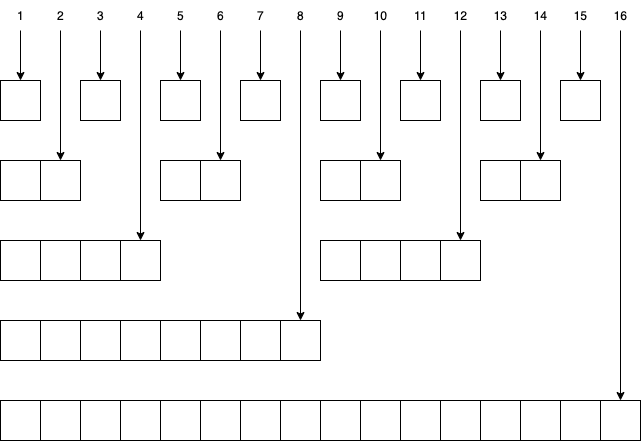
\includegraphics[width=\textwidth]{./Pictures/Pic1.png}
Man beachte den Start der Liste beim Index 1 und nicht 0. Für den Pseudocode wurde eine Indexierung von 0 angenommen, da dies näher an den meisten Programmiersprachen ist.
Wenn man dann $f(a_1,\dots,a_i)$ auslesen will, geht man wie folgt vor:\\
\begin{lstlisting}
f(FT, i) {
    res=iniatializeF //Default Value for f with no input
    //& is the binary AND operator
    for (; i >= 0; i = i-LSB(i)) 
        res = f(res, FT[i]);
    return res;
}
\end{lstlisting}
Für das auslesen braucht man einen Standardwert (res), der für $f(\phi)$ den Wert darstellt. Jetzt geht man in die andere Richtung wie beim Einsetzen vor, anstatt das LSB zu addieren, wird dies abgezogen und in jedem Schritt $res=f(res,FT[i]))$ bestimmt. Bei $11$ wäre dies dann $11\rightarrow 11-1=10 \rightarrow 10-2=8 \rightarrow 8-8=0$.






